In \Cref{sec:reconstruction_overview} it was discussed that in about a half of all reconstructed events there exists more than one tag-side candidate.
That does not take into account the overlap between \feiBp and \feiBz mode -- which further enhances this effect.
Performing the best tag-side $B$ candidate selection is important, as multiple entries per event should not be included in the final sample.
In this section, the definitions for best-candidate selection are discussed.
Furthermore, a concrete definition for tag-$B$ mesons with correctly reconstructed kinematic properties is introduced.

\subsection{Selection within the same \texorpdfstring{\FEI}{FEI} mode}

The number of tag-side candidates for \feiBp and \feiBz modes, after the optimised selections in \Cref{tab:cutflow},
is shown in \Cref{fig:fei_tag_reco_candidates_post_optimisation}.
Overall, comparing to \Cref{fig:fei_tag_reco_candidates}, the candidate fractions are similar -- which attests to the fact that background (and particularly continuum) suppression was done without introducing a bias in preferentially selecting events with large \feiProb.

\begin{figure}[htbp!]
    \centering
    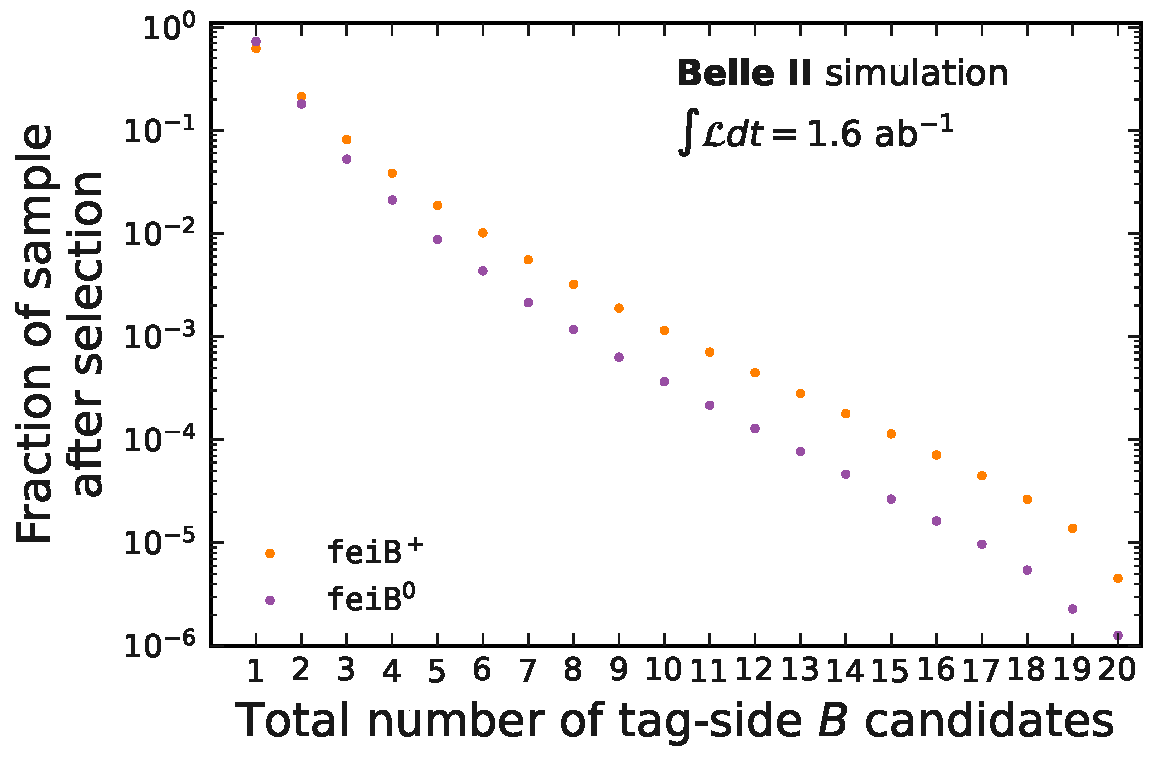
\includegraphics[width=0.45\textwidth]{figures/event_reconstruction/Bboth_total_tag_candidates.pdf}

    \caption{\label{fig:fei_tag_reco_candidates_post_optimisation} 
    Relative fractions of events for the number of \B meson candidates in the generic \MC dataset after the background suppression selections in \Cref{tab:cutflow}.
    This figure can be directly compared with \Cref{fig:fei_tag_reco_candidates}.
    The overall fractions are similar.
    About 67\%(74\%) of events for \Bp and \Bz \FEI modes have only 1 tag-side candidate.
    About 19\%(17\%) of events for \Bp and \Bz \FEI modes have two tag-side candidates and 7\%(5\%) has 3.
    The number of candidates per event reduces quickly, but faster for \Bz modes, with roughly 2\%(1\%) of events having more than 5 candidates for \Bp and \Bz.
    Note that the same event can have a \Bp and \Bz event reconstructed.
    }
\end{figure}

\todo[inline]{I should maybe make an argumen twhy picking highest rated FEI candidate is ok. Idea could be to make a plot of Fei sig prob for randomyl chosen and best and hope its similar.}